\chapter{WorkshopAR - Architectural Design \label{ch4}}

The following chapter will discuss the architectural design of \emph{WorkshopAR}, the educational software developed to explore the research topic of this thesis and to
gather data related to the research questions formulated. This and the following chapters are dedicated to the technical identity of this research and will discuss the
development process followed, the technical analysis done to accommodate the educational context of the development, the technical issues found through the design and
implementation stages, the results obtained and the path forward for future implementations.

This chapter will focus on the description and analysis of the conception and design stages of WorkshopAR, a prototype implementation and proof of concept of an \ac{AR}
technology for education. Specifically, the intention of this chapter is to discuss these  main points:

\begin{itemize}
    \item The architectural design of the software, the challenges that were present in the context of the research questions and the different solutions proposed to
    tackle them.
    \item The technology integrated into the proposal and used for the development process.
    \item The changes in approach and solutions that had to be made in response to the learning design context, the challenges posed by the selected technology and the
    data gathered during the testing stages.
\end{itemize}

As stated in Chapter \ref{ch1}, the educational pillar of the research has never been far from its software development counterpart. This is especially important in the
conception-design-implementation cycle used for the development of \emph{WorkshopAR}. It was essential to stablish the proper motivation behind the software development in
terms of educational research, its broader position in the field of \ac{TEL} and its more particular purpose in the context of the case study selected for this project.

Chapter \ref{ch1} also offered a detailed explanation of the research questions that motivate the construction of a specialised software. To summarise that information,
this thesis aims to identify what elements, unique to \ac{AR} technologies, can be used to enhance the classroom experience by offering benefits that are different or
comparable to other technologies. Through an extensive review of the literature, which was detailed in section \ref{sec:2-3}, four main factors that distinguish \ac{AR}
from other technologies emerged:

\begin{itemize}
    \item Visualising and interacting with abstract or difficult to come by concepts and objects.
    \item The ability to keep and incorporate the immediate context as part of the experience.
    \item A mobile-first deployment philosophy that eases development to an extent and proves to be more accessible to the end user.
    \item Easy integration with other tools in the mobile environment like cameras, movement sensors, GPS and ubiquitous connectivity.
\end{itemize}

The literature review showed that there is an increasing tendency to develop \ac{AR} applications that leverage the capabilities of a mobile hardware. Access to diverse
sensors detect the context and environment of the user and diverse image recognition tools are used to blend in it digital information that creates an experience that is
unique to \ac{AR}. Nonetheless, most educational apps are single-user experiences, which undermines the equally powerful connectivity tools provided by the mobile
ecosystem.

Multi-user \ac{AR} experiences (educational or not) excel the most at co-located, in-person activities. GPS-based augmentation is also used to create strong experiences in
shared spaces, building connectivity on top of a different framework in the mobile network infrastructure  and prioritising the sense of presence in a physical space
rather than an abstract connection with other users.

With this information it is possible to establish  one of the main motivations for the development of \emph{WorkshopAR}: to create an \ac{AR} application made for a
multi-user interaction that explores the technology's capabilities for digital visualisation, context awareness, seamless connectivity and a strong link to the physical
space shared by the users.

The literature review was also used to provide an analysis of the TEL field. It was possible to identify two problems that proved to be the most relevant for this project.

First, there is a clear trade-off when adapting any technology in the classroom between the benefits obtained and the issues that are related to the implementation, usage
and management of the technology. In this relationship between technological development and learning design, it is important to consider all the instances in which one
aspect informs the other, and it is even more important to be aware of all the issues that arise when there is a mismatch between both approaches.

Available literature also shows a lot of instances in which a technological development was poorly received. Many studies pointed out the dangers and inefficiencies of a
particular technology in learning scenarios, and it is possible to identify a push towards reconsidering the role of information technologies in the classroom
\parencite{boonmoh_2021,becirovic_2023,ifinedo_2021}.

The second area of motivation for WorkshopAR is to explore the synergy between the developer and the educator. Hopefully, the documentation of the design and development
process followed for \emph{WorkshopAR} provides valuable insight of the challenges of creating educative technology, to the point of becoming useful for future projects in
similar scenarios. A good step forward from this research would be to polish the positive experiences and to discuss the negatives in future work.

Section \ref{sec:4-1} of this chapter will provide a general description of the context in which WorkshopAR was developed and the broad requirements that were identified.
Section \ref{sec:4-2} will show a more detailed description of the use cases and scenarios designed for the tool and their relation to the overall research goals of this
project. Section \ref{sec:4-3} is dedicated to the architectural design of the software, focused on the high-level decisions taken to accommodate the learning goals
present in the development context and in the research objectives. Finally, section \ref{sec:4-4} offers a broad summary of the results obtained and the conclusions
reached from the analysis process made throughout the chapter.

\section{Project Description \label{sec:4-1}}

From exploring the literature, it was possible to extract the idea that \ac{AR} experiences build around the connectivity tools available in the mobile-based deployment
environment showed very positive results and interesting pathways for future research , but a lot of developments were not taking advantage of these tools. With those
findings in mind it seems fair to propose a software development using \ac{AR} interactions in a multi-user environment as an avenue to gather data and build a case study
that explores the use of technology that supports collaboration as a teaching tool.

By setting the development in the proper scenario, it is possible to analyse how students use \ac{AR} technologies as an aid for the collaborative aspects of their
projects. It would be of interest to identify what problems are the students solving or finding, how the technology shapes the structure of their work, the relationships
between peers or the development of their learning process. By comparing these observations with the behaviours of other students in the same scenario, it would be
possible to identify key behavioural changes promoted by the implemented tool, opening the possibilities for further analysis and pathways for future development.

In general, the development of WorkshopAR aims to fulfil three main objectives, which are independent of the learning goals proposed by the case study context. These
objectives will be labelled as Observation Objectives:

\begin{displayquote}
    OO1. Visualising my team. Sections \ref{sec:2-1-1} and \ref{sec:2-1-4} of the literature review exposed the challenges of teaching collaboration skills, and described the
    process in terms of the time, guidance, and exposure to proper tools needed to succeed. WorkshopAR is meant to use \ac{AR} to graphically convey the information needed
    to manage a group, for establishing a discussion or for organising a conversation. The idea is to offer tools that convey a good grasp of who the group members are and
    what they are doing.
\end{displayquote}

\begin{displayquote}
    OO2. Visualising decisions. \emph{WorkshopAR} should provide the ability to show digital representations of the learning material and allow the user to hold a
    discussion around that. The discussion can derive in solidifying knowledge or building learning, or could help in managing decisions, debates with peers or giving a
    visual representation to the workflow followed by the group. It should be possible to determine from the observations if interacting as a group with a digital
    representation of the learning material promotes any change on how the group is learning, how the material itself is being used, or if the augmentation helps managing
    the learning activity or not.
\end{displayquote}

\begin{displayquote}
    OO3. Augmenting the workspace. \emph{WorkshopAR} was initially envisioned as a tool for presential collaboration with a physical shared space where the students are
    working. The tool should be able to use that space as an anchor for the visualisations and use the capabilities of \ac{AR} to give extra meaning to that physical
    context, either by identifying and using elements of the environment in the augmentation or by adding digital elements anchored to the space that can help the user to
    create such meaning. In terms of research goals, observations should be able to identify if the ability to augment, visualise and customise digitally the physical
    environment of a group helps with aspects related to team identity, productivity or team management.
\end{displayquote}

So far, these objectives are devoid of context. Their aim is to support the research questions proposed, especially SQ1 to SQ3. The objectives describe activities common
in any collaborative situation, and the insights found in the case study can provide answers to questions related to the value of \ac{AR} in education. The main hypothesis
does state that \ac{AR} offer advantages using clever visualisations and quick interactions with the context, and \emph{WorkshopAR} is proposed to offer such scenarios.

\subsection{Context: Built Environments Industry Project Course \label{sec:4-1-1}}

Industry Project (ENBU 79X/89X in the university's enrolment system) is the final course offered for a variety of programs under the Built Environments department at
\ac{AUT}. This department includes the undergraduate programs of Architecture, Construction and Architectural Engineering, Civil Construction and Spatial Design.

ENBU 79X/89X is described as a multi-disciplinary course focused on providing an industry project experience that bridges the academical studies of the program and the
professional career of the students. In educational terms, this is a project-based course, providing the students a year-long case study that they must work out as a team
to provide a solution design, a construction plan, and an estimation of costs. The course does not provide a conventional curriculum or study plan, as it is mostly devoid
of content. Instead, the course acts more as a final opportunity to assess the skills and knowledge gained in previous courses, akin to a research project or thesis.
Nonetheless, the course has very clear learning goals:

\begin{itemize}
    \item Propose, organise, design, execute and reflect on a multi-disciplinary project.
    \item Apply existing knowledge and skills.
    \item Demonstrate initiative and independence in decision making scenarios.
    \item Deliver comprehensive client and progress reports.
\end{itemize}

The course has an overall focus on giving students opportunities to develop crucial soft skills related to teamwork, communication, planning and management. There is also
a substantial emphasis on developing the relationship between client and team in terms of communication, progress and stakeholders. All course assessments move around the
idea of reporting progress and decisions to the client. All elements of the project involve a two-way communication to understand views and requirements about relevant
policies, possible designs and bits of information needed for the proposals.

The course also promotes a strong multi-disciplinary approach. Four different roles are represented from the different bachelors that are part of the Built Environments
department: \ac{AE}, \ac{CE}, \ac{CM}, and \ac{QS}. Each role represents an important aspect of the project, and every team is composed of at least one representative of
each role. Every role has a particular set of goals inside the project and works towards specific learning outcomes. The project is built around constant communication
within the group, distribution of tasks, and effective collaboration to succeed.

In summary, ENBU 79X/89X is a course that focuses on developing crucial soft skills on students in the context of project development and management, emulating in
different ways common processes and scenarios found on the construction industry. In general, the learning goals can be enunciated as:

\begin{enumerate}
    \item Develop, document and communicate the design, plan and cost estimation of a construction project, considering the expectations of the client and the limitations
    exposed by the context, relevant policies and local constraints.
    \item Participate in and contribute to the project as part of a team, considering the expectations of the role as well as the processes and tools agreed upon by the
    group.
    \item Create and use the proper tools to communicate decisions to the client, report progress, receive feedback and ask for information.
\end{enumerate}

The course provided other set of particularities and complexities that made it a very interesting case study to explore in detail. All that information can be found in
Chapter \ref{ch5}. For this section, this is enough context to position the development of \emph{WorkshopAR}. The course provided an ideal scenario to test goals associated with
teamwork and \ac{CL}, as well as to provide the opportunity to have evidence of this process in all the stages of development of both a collaborative
project and a course, not only in an individual assessment or lesson.

With this context at hand, we can position \emph{WorkshopAR} as an educational technology development meant to offer support to the students of the Industry Project course
their coursework and the management of their team. It is possible then to elaborate on the educational and development goals of \emph{WorkshopAR} in relation to the
research questions of this thesis, which is the objective of the following sections.

\subsection{Learning Goals \label{sec:4-1-2}}

The expected learning outcomes for the Industry Project course highlight teamwork and communication, and as such, the intervention designed around \emph{WorkshopAR} should
focus on identifying the tools that \ac{AR} technologies can provide to facilitate or boost that collaborative process. The aim should be in facilitating group management,
communication among members and aiding in the production of knowledge and materials for the project.

The guiding prompt of \emph{WorkshopAR} is to provide students with a digital environment that helps in visualising the activities performed by the team and to highlight
possible tools at their disposal for proper team management, discussion of ideas and effective decision making.

By aligning these goals with those of the course, \emph{WorkshopAR} can provide a tangible feel of abstract concepts used in team management like participation, ideas and task
allocation. It can also reinforce in the students the need to develop a strategy to deal with issues related to groupwork. It can also prompt ideas about self-reflection,
evaluation of performance and the development of each individual role inside the group.

The main goal can also be aligned to research questions SQ1 through SQ3. The case study around ENBU79X/89x provides an ideal observation environment to compare different
approaches to collaboration, not only with those using \ac{AR} or not, but also behaviours related to the use of different types of technologies and to the circumstances
fostered by the design of the course.

Since the case study is complex and strongly based on observations, three scenarios have been selected to focus the development of \emph{WorkshopAR} and to simplify and direct
observations, comparisons and analysis, making the data gathering process manageable for the timeframe of the research.

These scenarios represent the general framework used to provide context to more specific and goal driven use cases in the future, which will be exposed in Section \ref{sec:4-3}.
The scenarios are born from the learning goals of the course but not necessarily from the particularities of its development. They represent common instances of
collaborative work and common roadblocks in the development of effective teamwork (see Section \ref{sec:2-1-4}). A deeper analysis of the implementation of the tool is
described in Chapter \ref{ch5}, and a description of the changes and adaptations needed to properly incorporate \emph{WorkshopAR} as part of the observed cohort of
ENBU 79X/89X can be found in Chapter \ref{ch6}.

\subsubsection{Scenario 1: Team Management \label{sec:4-1-2-1}}

The first scenario is about tools that can be used to manage the composition and dynamics of a group and to help in answering questions like: Who is my team? What are their
roles? What is my role? \parencite{bannister_2014,delgado_2008}.

The proposal is to use visual cues and digital constructs to represent information about team members and their work, offer the means to interact with such information and
to share it with others. This \emph{digital profile} can help students to start a conversation around the structure of the group and the evolution of the dynamics of its
members. The same reasoning can be applied to give a visual anchor to the tasks allocated and the roles assigned.

A specific manifestation of this scenario is the first contact the members of the group have. \emph{WorkshopAR} can help in that first process of identifying who is who, to
create the proper environment dialog and to establish the first rules of communication. It can also be extended to scenarios such as a new member trying to integrate into
the group or as a management tool to experiment and consolidate the group's structure.

\emph{WorkshopAR} can also provide a digital presence for the team itself and represent information about the work being done and who is doing it. This digital presence
can be defined in terms of the physical space where the group is meeting. This will serve as the positional anchor for all the digital constructs that can be used as part
of the team's activity. A digital room can be created for the team members to enter or connect which would signify the disposition to start working. The room will be
constrained or superimposed to the physical space where the group is gathered and can be composed by the digital constructs the team is using to work and all the physical
elements the application could recognise.

This is a good moment to explain the first design constraint taken for this project. \emph{WorkshopAR} will provide support only to face-to-face collaboration. Online or
asynchronous collaboration won't be considered.

Sections \ref{sec:2-1} and \ref{sec:2-3} of the literature review exposed the importance of network technologies in the analysis of \ac{CL} and the
expansive field of online collaboration. The opportunities of exploring the connectivity capabilities of mobile devices as part of \ac{AR} application was also part of the
discussion, and a big focus of this development is to explore such possibilities and to leverage the ubiquitous connectivity offered by mobile devices to power seamless
connectivity between users.

It is also true that this research wants to understand the unique capabilities provided by \ac{AR} technologies in terms of augmentation of the physical space, a scenario
that adapts easily to face-to-face interaction and connectivity with users in proximity. This does not mean that such elements cannot be together with online interactions,
but they do add another degree of complexity to both the research and the development of the software, risking the possibility of taking the spotlight from the main
objective of understanding \ac{CL} and the influence of \ac{AR} in the process.

To conclude, Scenario 1 proposes a solution in which the team and each of the team members have a digital profile that can be interacted with. The information in the
profile can be used as the main anchor for the software to provide the visualisation and augmentation tools that aid in the process of team management, communication,
roles, task allocation and team structure.

A visual representation of all these concepts can be seen in Figure \ref{fig:4-1}, where the room represent both the physical space used by the group to work and the
current instance or session the group is participating in. The room will hold all the digital objects used during the session as well as framing all the other activities
the team can perform.

\begin{figure}
    \centering{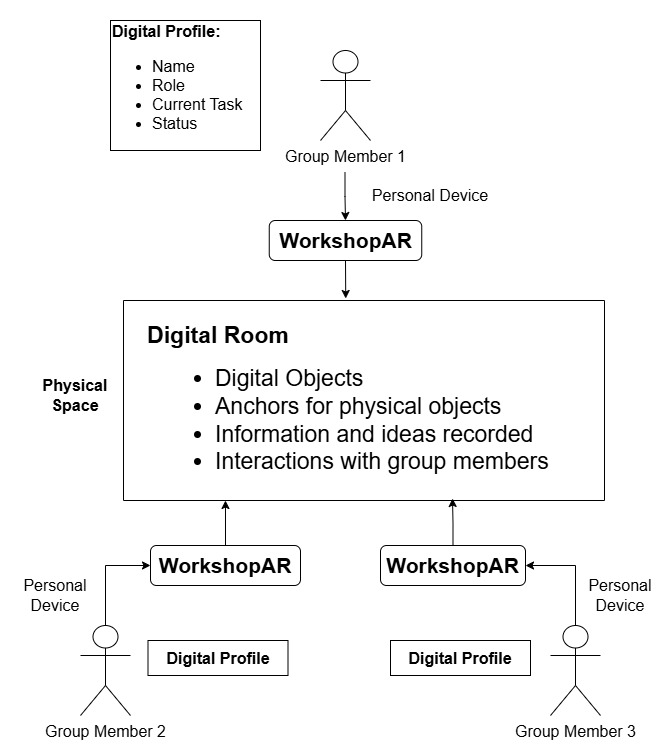
\includegraphics[scale=0.6,alt={Figure 4.1}]{figures/F4-1.jpg}}
    \caption{Team Management Scenario \label{fig:4-1}}
\end{figure}

\subsubsection{Scenario 2: Work Session Management \label{sec:4-1-2-2}}

For this scenario, we can define a work session as an activity the group decides to execute for a given time with a set of goals in mind. It can also be described as the
group members participating in a lesson or a learning activity. The session would be composed by participants, the space the session is taking place in, and the goals
proposed.

It is envisioned that \emph{WorkshopAR} can provide tools to identify and manage aspects like:

\begin{itemize}
    \item The participants in the work session.
    \item Status of the session.
    \item Current objectives and the status of those objectives.
    \item The resources at hand for the session.
\end{itemize}

Scenario 1 is about giving the room a digital representation that can be interacted with. Scenario 2 uses those elements to construct a digital representation of the work
session, as shown in Figure \ref{fig:4-2}. The participants will connect to an active room in which a session is taking place. The room will be associated with a set of
goals, active resources and a physical space to which is anchored.

\begin{figure}
    \centering{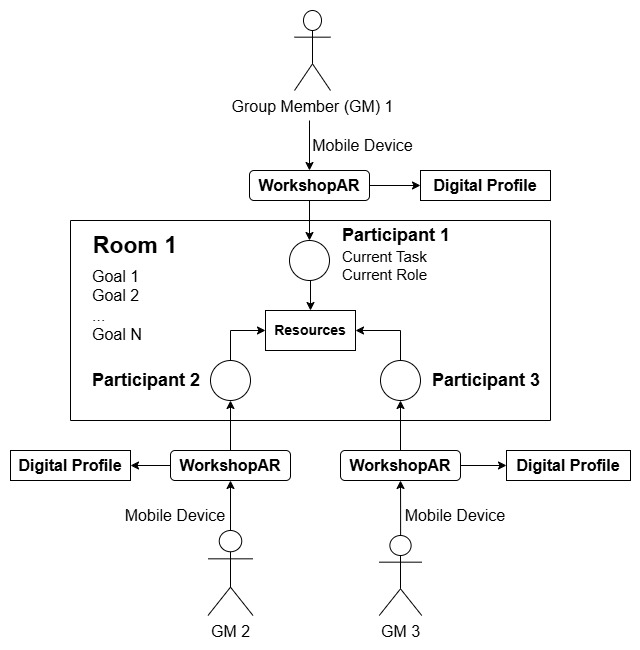
\includegraphics[scale=0.6,alt={Figure 4.2}]{figures/F4-2.jpg}}
    \caption{Work Session Management Scenario \label{fig:4-2}}
\end{figure}

The second development constraint that can be analysed at this stage is related to resources. Ideally, WorkshopAR should be able to provide or interact with all the
resources the group needs to perform their work. In just the context of ENBU 79X/89X, the list of available resources could comprise elements such as:

\begin{itemize}
    \item Tools for creating documents and presentations.
    \item Tool for architectural design and analysis.
    \item Spreadsheets for calculations and project management.
    \item Visualisation of documents and design proposals.
    \item Tools for digital modelling and design.
\end{itemize}

It is not feasible for the scope of the development to consider all the possibilities. Seamless interaction between tools is a valuable quality functionality but would not
add significant insight into the research goals at hand. In contrast, observing how the students interact and integrate all the technological tools at their disposal, and
how they evaluate their usefulness and functionalities, does align with the observation objectives of the research, providing insights for questions SQ4 and SQ5, which are
trying to identify the specific value of \ac{AR} in learning scenarios, especially in comparison to other tools.

\emph{WorkshopAR} will be limited to two resources that can be used as part of a working session:

\begin{enumerate}
    \item Visualisation of and interaction with simple digital models for planification and discussion.
    \item Anchoring data or information to a digital object or physical space.
\end{enumerate}

These two resources offer general help for the most common activities of the course: proposing solutions to the spatial design of the project and organising discussions
around such proposals. The purpose is to analyse how the students change (or not) their approach to collaborative work when they have access to more tangible
representations of abstract concepts such as ideas, proposals and discussion, and how (if at all) the discussion is affected by the ideas being more visually anchored to
the real world.

\subsubsection{Scenario 3: Discussion and Debate Management \label{sec:4-1-2-3}}

Scenario 3 is related to the activities that can be performed during a work session but that are not part of the team management. \emph{WorkshopAR} aims to offer tools for
discussions and debates around the work done by the group and the decisions being taken. The tool can give visualisation and structure to elements like:

\begin{itemize}
    \item The object of debate or discussion.
    \item The structure and flow of the discussion.
    \item The responses and ideas generated.
    \item The active participation of different team members.
\end{itemize}

The proposal is that \ac{AR} can offer a visual anchor or structure to the process, helping students in understanding it and managing its flow.

To summarise, the three scenarios presented above illustrate the main learning objectives guiding the design of \emph{WorkshopAR}. The objective is to provide a tool that
helps the students to identify and structure the most relevant aspects of their collaborative work such as team management, work management, communication and decision
making.

\subsection{Development goals \label{sec:4-1-3}}

It is also possible to identify a set of points related to the technological and software development of \emph{WorkshopAR} that are worth analysing and that can offer
insights on how the technology influences the achievement of the learning goals. Some constraints in the development process can also be discussed related to issues
highlighted in this section.

The first development goal is concerned with the multi-user \ac{AR} experience. This requirement implies some form of network infrastructure to support several users
interacting at the same time, sharing resources and visualisations. Thanks to the information provided on the descriptions of scenarios 1 through 3 in the previous section,
it is possible to summarise the main extent of the networking development into the following objectives:

\begin{itemize}
    \item Provide a lobby-like architecture for connectivity, allowing users to connect in and out of a work session in a seamless way.
    \item Share and synchronise information about the digital profiles of the team, the room and the resources being used.
    \item Share a synchronous interaction with the digital objects used and the augmentation created for the work session.
\end{itemize}

The main proposal of the research is not the software solution developed, rather the interaction design engineered to fulfil the networking requirements and the process
followed to integrate the solution in the flow of a work session, considering some important requirements imposed by the context of the case study:

\begin{itemize}
    \item Offering a seamless connection with minimal or high-level configuration.
    \item Disrupting the work of the students as little as possible, considering they are contributing to a graded project that is part of their professional education.
\end{itemize}

The second development goal is to provide a platform-independent solution that can support a \ac{BYOD} approach to the implementation of technology in the classroom
\parencite{disterer_2013}. This considers that, in theory, the main platform for deployment of \ac{AR} solutions are mobile technologies, an ecosystem that is ideal for
\ac{BYOD} initiatives \parencite{imazeki_2014,valjataga_2016} due to accessibility and ubiquity. Mobile devices also offer hardware solutions to several of the networking
objectives proposed previously.

Additionally, a solution that is platform-independent can also aim to accommodate \ac{AR} devices that are not based specifically on smartphones, such as specialised \ac{MR}
headsets like the Meta Quest 3, Magic Leap or the HoloLens. This would create a challenge in design to adapt the control and interactions of the experience specifications
that each participant has access throughout a session. Figure \ref{fig:4-3} shows a high-level architecture of a possible solution for this scenario, which is similar to
other systems that offer cross-platform functionalities, commonly across a web deployment \parencite{medvidovic_2002}.

\begin{figure}
    \centering{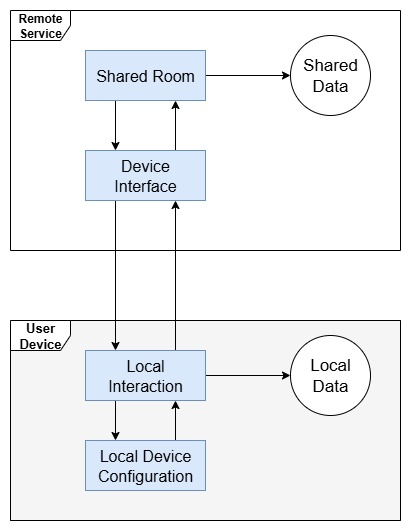
\includegraphics[alt={Figure 4.3},scale=0.8]{figures/F4-3.jpg}}
    \caption{Concept of a Multi-Platform Architecture \label{fig:4-3}}
\end{figure}

Similar to the way in which systems like Netflix balance access to content depending on the device used for access \parencite{netflix_2023}, a general architectural proposal for
\emph{WorkshopAR} would consider an interface between each local participant and the shared interaction in the room. The interface can manage input interactions, data
types and visualisation types before handling control to the shared room, and vice versa, handle responses and transform them to data that can be properly processed by
every device connected to the session, akin to a system like \textcite{andres_2017}.

With that analysis in mind, Chapter \ref{ch5} will describe in more detail the reasoning behind not  pursuing a full cross-platform architecture. In summary, the research
value did not align properly with the value gained by this type of development. The \ac{BYOD} approach was instead tested by focusing on mobile devices which, paired with
other technologies selected for the development, already covered any mobile architecture using Android or iOS, offering a wide spectrum of devices available to the users.

The one element left behind by not pursuing a full cross-platform architecture was testing the integration of different means of interaction in the same work session. It
was decided that, for the scope of the research, it was worth to focus first on other aspects of the development and probably relegate this aspect for future work.
Nonetheless, the question of cross-platform will resurface in the analysis of the case study and during the user-centred design described in section \ref{sec:5-1-1}.

In conclusion, the development of \emph{WorkshopAR} proposes architectural and implementation solutions for a multiuser \ac{AR} application deployed over cross-platform
mobile technologies. These objectives provide opportunities to understand the technological challenges of implementing multiuser \ac{AR} applications and how they affect
and are affected by the learning goals proposed previously.

\section{Use Cases \label{sec:4-2}}

The scenarios described in the previous section represent the general goals for which WorkshopAR will be used as an intervention in a learning setting. To start the
software design process, the first step is to identify and describe the specific functional requirements to be developed. The following section will describe the most
relevant requirements identified for the research intervention of ENBU 79X/89X. This information is going to be described in the form of use cases, or user stories, to
emphasise three aspects:

\begin{itemize}
    \item The general interactions performed by the users, not the particularities that have to be developed.
    \item The development goal being fulfilled by the use case, or at least any technological challenge that could be of interest for the analysis process.
    \item The learning goal being fulfilled and how it is related to the educational objectives of the research.
\end{itemize}

Before exposing the use cases, it is necessary to discuss some of the vocabulary that is going to be used in the descriptions. These are terms referring to common elements
of the interaction with the app, the activities enabled by it and the resources used to create the experience.

A \emph{user} is any student using the app. Every user has a personal profile that is shared between sessions. Although in the context of ENBU 79X/89X all students belong
to a particular group for the development of the course's project, the app is not going to enforce that organisation, and a user can become a participant in any session
available.

A \emph{participant} is a user that has joined a \emph{digital room} and now is part of a \emph{work session} with other users. As a participant, a user has a role and a set of assigned
tasks, which are only valid inside a particular session.

A \emph{digital room} is the space created by the app and used by the participants to hold the session. The room doesn't need to be a closed space. The app creates a
\emph{workspace} for the room and associate the session information to a room anchor, a digital object situated in the space selected.

A \emph{work session} is the work done by the participants that enter a \emph{digital room}. The session has a general goal associated, which can be modified and updated.

A \emph{workspace} is a digital object representing a space in which the participants can position and interact with digital objects. In conjunction with the \emph{room anchor},
it also creates a visual representation of the \emph{digital room} in which the \emph{work session} is taking place.

\subsection{Create a Shared Digital Room \label{sec:4-2-1}}

\textbf{Description:} A user must be able to initiate a \emph{work session} by creating a new \emph{digital room} for the group. The \emph{digital room} is identified by a unique
name and described by a set of goals for the session. The user can configure all these elements before launching the session. Upon opening the \emph{digital room}, any
other user can search the name of the room and join it, adding themselves as participants to the \emph{work session}.

A \emph{room anchor} will be added to the \emph{digital room} which will present information about the \emph{work session} upon interaction.

\noindent
\textbf{Development goal:} The \emph{digital room} represents the main point for the multiuser experience. All the participants in the \emph{digital room} will share the
same visualisations and will be able to interact simultaneously with the same digital objects. Ideally, the connection to the \emph{digital room} is seamless, requiring
only the initial configuration for setup and run.

\noindent
\textbf{Educational goal:} The \emph{digital room} will be linked to the concept of a \emph{work session}. When a room is active it means that the group is working, and all
the participants share a current goal. The \emph{digital room} provides the students the opportunity to have a structured \emph{work session}, and the digital markers
used provide a tangible and interactable representation of the goal and the room itself.

\subsection{Create a Shared Workspace \label{sec:4-2-2}}

\textbf{Description:} Upon creating a \emph{digital room}, a participant needs to define a space in the physical environment that will be used as the shared \emph{workspace}
for the session. \emph{WorkshopAR} will identify suitable horizontal spaces like tables, desks or the floor, and overlay a digital plane over them. The participant can
select one of the detected planes and modify it to convenience to suit the preferences of the group or the needs of the current session.

\noindent
\textbf{Development goal:} The \emph{workspace} will be the base augmentation provided by \emph{WorkshopAR} to give a visual representation to the \emph{digital room}. The
\emph{room anchor} gives basic information about the session, while the \emph{workspace} facilitates the interactions with other digital objects, constraining the movement
and location of all the interactive 3D models and providing a reference point for any other digital constructs.

\noindent
\textbf{Educational goal:} The \emph{workspace} gives a location for the shared resources of the group, elements that are public to everyone and could be used as inputs in
each task. The \emph{workspace} anchors all the digital objects to a common point and the group itself, creating a visual representation of the \emph{digital room} while
keeping the constrains of the physical space used. These constraints are more malleable than in a normal room, and the group can use the digital elements of the app to
explore or expand what is provided by the physical space.

\subsection{Create a Profile \label{sec:4-2-3}}

\textbf{Description:} A user can create a digital profile to use in a \emph{digital room}. The profile is linked to the instance of \emph{WorkshopAR} installed on their
device. When not connected to a \emph{digital room}, the profile consists of a preferred name and a colour that represents the user. When connected, a user can also be
described by a role and a set of current tasks.

\noindent
\textbf{Development goal:} The profile is a representation of the users in the when connected to a \emph{digital room}. It also serves as an anchor for interactions with
other participants and provides a form of digital avatar that carries the information of the profile.

\noindent
\textbf{Educational goal:} The participant's anchor gives visual structure and prompts the discussion around different topics like team management, assigned roles and
allocation of tasks.

\subsection{Point to Something or Someone in the Digital Room \label{sec:4-2-4}}

\textbf{Description:} This case is related to provide basic communication tools to the students, specially to convey information about the resources available and the
users connected to the \emph{digital room}. Participants should be able to specify the person or object (physical or digital) they are referring to in a conversation or
instruction. This clarification in the communication process is going to be referred as \emph{pointing}.

\noindent
\textbf{Development goal:} This interaction is meant mostly for digital objects and has an important role in the multiuser experience. It is a simple tool to facilitate
communication and helps to mitigate any ambiguity or confusion. It is also an interesting technical challenge to account for both digital objects and the physical context
of the room. 

\noindent
\textbf{Educational goal:} This is a simple tool to promote and facilitate communication. It is one of many ideas to explore the concept of \emph{augmented collaboration}
by providing digital tools to visualise the communication process and analyse its impact in the behaviour of the students regarding learning, group dynamics and team
management.

\subsection{Check the Status of Other Participants \label{sec:4-2-5}}

\textbf{Description:} A participant should be able to access information about everyone connected to  the same \emph{digital room}. This information is related to their
profile and their status, described by their role, assigned tasks and participation state in the activity.

\noindent
\textbf{Development goal:} The technical challenge of this use case is related to the way the information present in the profile can be transmitted and synchronised on the
network, as well as the proper interaction methods to access it. These interactions can also be extended to accessing the information and current state of the \emph{digital room}.

\noindent
\textbf{Educational goal:} This is an opportunity to understand the role and influence of technology as part of the collaboration process. Ideally, the tool provides quick
access to information about the current state of the session and the team members, but it could also become an unnecessary barrier for something that should be verbally
communicated. It should be possible to observe how students use this functionality, how it affects different communication processes inside the group and how \emph{WorkshopAR}
compares to other IT tools that mediate in communication.

\subsection{Share and Pin an Idea \label{sec:4-2-6}}

\textbf{Description:} A participant should be able to type an idea and pin the text representing it somewhere in the \emph{digital room}, making it public and accessible
to all the other participants. Similarly, a user should be able to see and interact with all the ideas pinned by them and other users.

\noindent
\textbf{Development goal:} This use case also belongs in the \emph{augmented collaboration} category and offers the opportunity to record and visualise ideas and
information in the same way a whiteboard would do. This is a way to experiment with the idea of offering a relationship between the digital representation of the
information and the physical space \parencite{zund_2015,wang_2017}. The objective is to prompt discussion, associations and structure to a conversation while sharing and
recording ideas between participants.

\noindent
\textbf{Educational goal:} In the same spirit, it is another tool to visualise and interact with information, making communication visible. The idea is that, by adding a
relationship between the space of the conversation and the ideas proposed by the group it will open the possibilities to get deeper, different or more structured types of
discussions.

\subsection{Add and Interact with a Model in the Digital Room \label{sec:4-2-7}}

\textbf{Description:} This interaction is related to simple digital models either build in external tools and imported to \emph{WorkshopAR} for visualisation or built in
the tool using simple construction blocks. Since the main objective of ENBU 79X/89X is related to architectural design, this interaction with digital models is meant to
facilitate communication and discussions related to this field. This communication can be centre d around collaborative creation of a design or discussing ideas, getting
feedback or proposing changes. This use case considers all the interactions needed to add the models to the app, share them in the \emph{digital room} and perform simple
interactions with them like moving, selecting and transforming (e.g., moving, rotating, scaling) the models.

\noindent
\textbf{Development goal:} More than a technical challenge, the focus of this use case is on the interaction design needed to propose a solution. For one, there is an
interesting opportunity to analyse the design and usability of the interactions needed for this task, considering that the app will use a mobile phone deployment. A set of
conventions in interaction and visual language are expected for both the selected hardware and the AR nature of the tool, and it is important to analyse those conventions,
implement them, expand them or revaluate them if needed.

Second, this interaction must consider the multiuser scenario of the project and the necessity to coordinate interactions of shared objects over the network. Although the
technical implementations of these requirements are interesting, it is more important for the research goals to observe how the user experience proposed forces or promotes
different behaviours in the users, and how those behaviours affect the learning and collaborative processes.

\noindent
\textbf{Educational goal:} The interaction between participants is again the focus rather than the activity itself. Since the main objective of the course was design and
construction planning, it was considered interesting to provide a flexible enough interaction that promoted discussions around different elements of the design process and
the ideas proposed by the students around space and structures. The building blocks metaphor was chosen to promote a visual and physical anchor of those elements of the
architectural design as part of the \ac{AR} experience.

A more explicit goal for the development of this functionality is to organise and structure the work of the students around digital and physical tools that boost the
idea-discussion-decision loop with \ac{AR} and communication technologies. This is, again, guided by the principle of augmented collaboration.

\subsection{Participate in a Debate or a Vote \label{sec:4-2-8}}

\textbf{Description:} A participant must be able to propose or be part of a group vote or debate. Both cases will be defined as instances in the \emph{work session} in
which the input of the participants is needed to take a decision. A vote is a decision to be taken among a possible group of options, while a debate has an open input
nature.

\noindent
\textbf{Development goal:} This is an interaction design that allows the users to visualise in the augmented space all the elements taking place in the decision-making
process. This idea explores possible implementations for the tool to manage a debate and to storage, compile and show the results of the activity.

\noindent
\textbf{Educational goal:} This use case reinforces the most prominent activities in which communication skills are developed thanks to the classroom groupwork. \emph{WorkshopAR}
is not expected to be used as the sole manager for the communication and planning needs of the group, as other tools probably already fulfil those roles. The idea is to
offer a different approach to the communication interactions that happen when taking decisions, specifically in face-to-face scenarios. This type of discussions is prone
to be more informal, unstructured and with no archive of the activity itself. Once more, the aim is to offer a different type of solution based on visualisation and
context augmentation.

\subsection{Pause the Current Participation \label{sec:4-2-9}}

\textbf{Description:} A participant should be able to signal the group that he/she is not actively participating in the session and that progress in the current tasks is in pause.

\noindent
\textbf{Development goal:} The reasoning behind this use case is to create a distinction between the physical presence of a participant in the \emph{digital room} and
their activities in the group, giving more depth to the status of a participant, also helping to visualise and symbolise some social cues that are hard to verbalise. In a
more technical sense, it is also a function that helps in pausing the use of the device without finishing the session.

\noindent
\textbf{Educational goal:} This option is the best example of a tool for group management that has more significance than simple actions like checking a list of
participants or managing access to the digital room. This functionality aims at giving visual presence to the work of the user, to establish boundaries, proper
communication habits and prompting discussions around time and space management.

\subsection{Conclusions \label{sec:4-2-10}}

The exposed use cases represent the most important functionalities that \emph{WorkshopAR} should be able to fulfil to provide insights for the research goals of the
project. These scenarios present the most common instances in which the students can develop collaborative skills or in which their collaborative work is the key aspect of
their work. These actions include diverse aspects of activities such as team management, task planning, effective communication and decision making.

The main proposal that this software development is meant to explore is that through \ac{AR} it is possible to create a visual representation of the work that the users
are doing and of the resources in use. The plan is to design simple interactions that create a relationship between the ideas explored with the tool and the collaborative
skills that the students need to develop.

The plan also relies on offering the proper environment to think or discuss issues around the structure used to work and plan, rather than to force a specific way of
working. This approach can create the opportunity for students to reformulate their current way of working and find alternatives that incorporate new information into
their processes, but it can also cause the students to completely ignore the tool.

This is an acceptable risk scenario. In first instance, it creates the least amount of friction with the teaching approach of the course, giving the students a technology
that they can freely use to enhance their work, and not a forced experience they could resent or that can even inhibit their work. It was decided that a free exploration
of the tool offered a better and healthier experience.

It is also acceptable in terms of the research goals. A scenario in which a group did not interact with the tool also offers interesting insights. Paired with the case
study, a failure engagement with \emph{WorkshopAR} can elicit questions regarding the tools that the group is using for communication and planning, how the group is
structuring their work and managing their time, among other possibilities. Answers to these questions can help in constructing an interesting case study.

\section{Architectural Design \label{sec:4-3}}

The following section will discuss the main ideas guiding the architectural design of \emph{WorkshopAR} and the reasoning behind the decisions taken. The whole process 
ill be described using the most important quality requirements identified for the development of the tool, the most important functional components designed, and the
available frameworks and technologies selected to help in the construction of the tool. For this purpose, several architectural and structural diagrams were created to
explain and visualise the design decisions taken and the software architecture discussed throughout this section.

A common visual language was used that loosely follows the structure and rules proposed by UML, but it was not strictly followed nor are any of the diagrams in this
section UML-compliant. The main objective was to offer a quick visual representation of software components and behaviours that facilitated the communication of concepts
and the discussion of the decisions taken, while keeping the diagrams simple and easy to read. The main rule was to keep consistency between diagrams, especially with
colour coded information as follows:

\begin{itemize}
    \item \sethlcolor{lightgray}\hl{Grey} elements represent hardware and devices, physical instances where software is deployed.
    \item \sethlcolor{yellow}\hl{Yellow} elements represent software components, entities or a set of entities that have a common purpose and functionality. They could be
    zoomed-in for more detail, but that is not necessary to understand the idea conveyed by the diagram overall.
    \item \sethlcolor{cyan}\hl{Blue} elements represent more abstract entities, either because they represent big complex functionalities which serve several purposes or
    because they represent a state or logical concept in the execution of the software that is achieved by the interaction of several other components. As with yellow
    elements, the component can be described in more detail, but it is not important or necessary for the purposes of the  diagram.
    \item \sethlcolor{green}\hl{Green} elements are specific instances of an object (a class or a game object in Unity) used to show the composition of an important scene
    or the flow of data in a use case scenario.
    \item \textbf{White} elements are used for data or information being used, created or transmitted between other software components.
    \item \textbf{Arrows} are used to signify relationships and associations between components, or messages sent from one component to another, depending on the context
    of the diagram.
\end{itemize}

\subsection{Quality Requirements \label{sec:4-3-1}}

\emph{WorkshopAR} is a prototype that helps in promoting proper work habits in the students for communication and collaboration. Independent of the specific functionalities
to be built, the software needs to achieve these objectives through the architectural design proposed:

\begin{enumerate}
    \item \textbf{Multiuser interaction:} \emph{WorkshopAR} is a cooperative experience for the synchronous interaction of small groups of 2 to 6 students. All the
    participants in the interaction will be present in the same physical space and will share the same digital augmentation of the environment, but with different points
    of view and instances of interaction. Digital objects in the space will also be shared and interactions with them must be synchronised and coordinated between users.
    The participants will have a digital presence in the shared environment that can also be interacted with, and that interaction also needs to be synchronised and
    coordinated.
    \item \textbf{Multi-platform deployment:} To support a \ac{BYOD} approach, it is necessary to build a solution with a multi-platform deployment. \emph{WorkshopAR} must
    work independent of any specific mobile platform and aim for the most common \ac{AR} capabilities of devices currently in the market. Ideally, the tool should also
    support any other \ac{AR} capable device, specifically, headsets available in the market like HoloLens, Magic Leap or Meta Quest 3. This implies that the tool must
    consider all the diverse input methods available, display varieties and processing capabilities, and coordinate them within the shared experience.

    This idea can be also expanded to a multi-role interaction, in which the activities are taking place in a room, consider different roles that any participant can take,
    and tailor how the user sees information and participates in the experience in accordance with that role. Different roles also open the possibility to interact within
    the room through mediums that are not necessarily \ac{AR}.
    \item \textbf{Spatial interactivity:} Due to the multi-platform approach taken and the irregular nature of the \ac{AR} capabilities found in current available devices,
    it was necessary to make decisions about the minimal capabilities needed for the \ac{AR} experience to function across different devices. It was decided that the core
    experience was in the augmentation of the communication process, and the relationship built between the group and the \emph{workspace}. It was necessary to identify minimum
    features common in most devices and decide which aspects of the experience could rely on the available technology and tool, and which needed a solution through a more
    complex development.
\end{enumerate}

The following quality requirements are not directly related to the outcomes needed for the research goals but are equally important to support a good development flow or
to accommodate the particularities found in the execution of the case study.

\begin{enumerate}
    \setcounter{enumi}{3}
    \item \textbf{Flexibility:} Given the interactive nature of the development proposed and the exploratory approach of the research, the general component architecture
    of the tool needs to be as flexible and decoupled as possible. Particularly, it is important for the input system and interaction methods and processes to be easily
    swappable without affecting the core functionality of the software. These are the most fluid elements of the design, and from the very beginning, they are meant to be
    part of the main experimentation with the software. A flexible approach is necessary to facilitate testing and different ideas and approaches.

    Solutions related to the network communication and the creation of a shared space also needs to be flexible. Ideally the main utility of the tool is independent of the
    networking architecture.
    \item \textbf{Extendibility:} Independent of the differences between the design and the implementation, component development will aim for cohesion and extendibility.
    The purpose is to support a small and incremental development that is easy to extend into full functionality over time. This will also support the user-centred
    approach proposed, where the users can experiment with a simpler version of a functionality, provide feedback and incorporate that information in the extension and
    refinement of the functionality.
    \item \textbf{Easy-to-learn:} One of the core issues identified in section \ref{sec:2-2-3-2} in the implementation of \ac{AR} in classroom is the all the extra time
    needed for students to learn the proper use of the tool. Lessons and plans had to accommodate, sometimes unsuccessfully, enough time to teach how to use the tool,
    coordinate its use in the planned activity and solve issues appearing when mishandling the tool.

    This issue is a complicated task worthy of its own focus research. The design of \emph{WorkshopAR} can leverage the common knowledge that students possess of their
    phones and the common interactions with them to propose interactions that emerge from the natural use of the technology. This can be achieved by exposing the users
    to small samples of the software and incorporate a systematic analysis of their feedback in the design process.
\end{enumerate}

It was important to follow a formal approach to the analysis and development of the easy-to-learn design, taking decisions based on principles found in the literature and
approaches proven successful in similar scenarios. The most relevant guiding principles are based on the work of \textcite{wigdor_2011} who state that a design based on
natural interaction is characterised by:

\begin{itemize}
    \item The feel of a natural extension of the body.
    \item Offering the same natural experience for novice and for expert users.
    \item An experience tailored for the medium (mobile devices), not a mimicry of the real world.
    \item The proper use of context, previous knowledge, metaphors and input/output devices.
    \item Using paradigms when needed but not being afraid to ignore them.
\end{itemize}

Other ideas were summarised from works like \textcite{macaranas_2015,strijbos_2004,good_1984} that state general good approaches such as:

\begin{itemize}
    \item Test different metaphoric mappings depending on the content of the interaction.
    \item High usability is achieved through careful analysis of feedback.
    \item Manage and consider user's expectations and knowledge.
    \item The changing expectations of the participants depending on the context of the experience and the tools available for the interaction.
\end{itemize}

\subsection{Technological Frameworks \label{sec:4-3-2}}

A set of tools were selected to implement current available technologies and frameworks to simplify the constructions of the basic functionalities of the application,
support the solutions for more complex problems and provide a pipeline for testing and deployment. The tools selected helped in the implementation of basic \ac{AR}
functions and worked as stepping stones for more complicated interactions, for the networking development and for the multi-platform deployment.

The Unity engine was selected as the main building platform. Similar to other tools and environments like Unreal and Godot, the initial use case of Unity is in the
development of videogames, but the tool can also be adapted to be the engine behind any type of multimedia interaction software \parencite{hussain_2020,codemonkey_2024}.
Unity was selected due to convenience and to leverage previous expertise with the tool.

Unity was used to handle the implementation of digital content and the interactions with it. Unity also helped in the management of diverse input methods and the
multi-platform deployment of the software. Some of the issues related to networking were also solved using the Netcode utility. This package allows for basic network
configuration and provides a framework to communicate information or to coordinate states of the objects across a network.

Finally, one of the biggest advantages of using Unity (and other similar tools) is that it provides an implementation of the OpenXR framework \parencite{openxr_2016}.
This framework is and open-source implementation that abstracts into a common language all the specifics of different \ac{VR}, \ac{AR} and \ac{MR} devices in the market.
OpenXR provides a platform-agnostic implementation of different features like tracking management, display, environment tracking, input handling, among other things. This
is a useful tool that helps in maintaining a single code base for the application and easily deploys it on different platforms at the same time. The project can then focus
on solving specific problems without having to deal with issues at the hardware level.

Additional to the tools provided by the Unity engine, two other frameworks were integrated to the development to help with functionalities related to \ac{AR} and the
shared interactions in the network, as described in the following sections.

\subsubsection{ARFoundation \label{sec:4-3-2-1}}

ARFoundation is an implementation by Unity that provides a similar level of abstraction as OpenXR but specifically tailored to the \ac{AR} environment and the mobile
devices ecosystem. This is an important tool that helps in dealing with the most important frameworks in the market for \ac{AR} development: ARCore and ARkit for Android
and iOS devices respectively. These two frameworks cover most of the mobile devices available in the market, while more specialised technology uses APIs or frameworks that
are either a derivation of the two main ones or can be handled with the OpenXR framework.

ARFoundation strongly influences the architecture of \emph{WorkshopAR}. ARFoundation provides a set of manager utilities that act as a front-end configuration for several
common functionalities of \ac{AR} such as image processing, feature detection, point-of-view tracking or image composition. The managers communicate with a series of
subsystems that abstract the specific hardware implementations of ARCore, ARKit or other similar toolkits. This means that all the functionalities of \emph{WorkshopAR} are
built by coordinating the managers provided by ARFoundation with the proprietary code developed for the application. Additionally, any implementation communicates with the
hardware layer via the subsystems available, allowing the creation of a single code base for every platform. Figure \ref{fig:4-4} shows the component architecture of
\emph{WorkshopAR} when deployed in a generic mobile device, differentiating between the code found in the core Unity implementation vs the local toolkit used to provide \ac{AR}
functionalities in the device.

\begin{figure}
    \centering{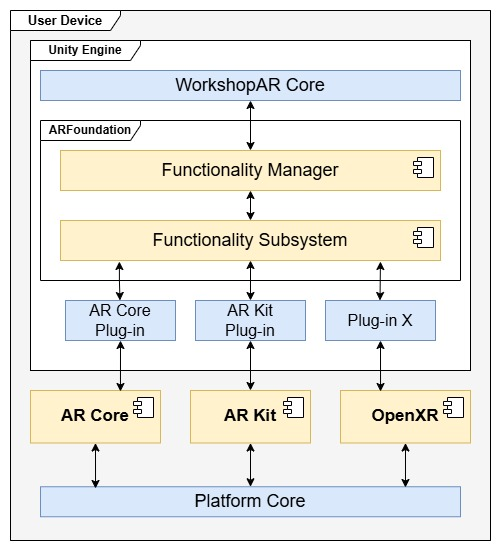
\includegraphics[alt={Figure 4.4},scale=0.7]{figures/F4-4.jpg}}
    \caption{Integration with ARFoundation \label{fig:4-4}}
\end{figure}

This solution facilitates a deployment that is, at least in theory, independent of any platform. In practice, it is not that simple. It is possible to support any mobile
device that implements ARCore or ARkit, and there is also the possibility to deploy in any other \ac{AR}-capable device if there is a subsystem in the ARFoundation toolkit that
supports it or if the device supports the OpenXR framework. The problem is that all these implementations do not communicate smoothly, and to support a proper
platform-agnostic single code base, it is necessary to identify all the intended platforms that are going to be used and coordinate all the low-level communication
elements of the code to properly function. Other element to consider is that if used as-is, ARFoundation only offers functionalities exposed by the managers, which can
obscure more updated versions of the lower-level systems or not show them at all.

\subsubsection{Lightship \label{sec:4-3-2-2}}

This component is part of the Niantic Spatial SDK suit \parencite{niantic_nodate} and the set of solutions present in the Shared \ac{AR} product \parencite{shared_nodate}. Niantic
has pioneered the commercial use of \ac{AR} in mobile environments through successful implementations in entertainment, educational and industrial contexts \parencite{lee_2022,bowtiedrobin_2021}.
The SDK offered through Niantic Spatial is a set of solutions compatible with most development environments to create and manage complex \ac{AR} interactions like life
meshing, semantic detection, complex image recognition and networking.

For the development of \emph{WorkshopAR}, the component integrated into the architecture is Lightship, a tool for the creation of shared \ac{AR} experiences without the
need of a complex backend network infrastructure. This tool is meant for small scale connectivity, supporting up to ten concurrent users. Lightship eases the development
of the multiuser requirements and offers a scalable and flexible architecture that can be expanded and build upon in future work.

In isolation, Lightship works by using a simple client-server architecture. Any instance of Lightship can be connected to another one through an internet connection if
they are using the same application ID. The architecture allows for the implementation of a dedicated server that controls the experience or for a distributed connection
with one of the client instances acting as a host. At the network level, it is possible to use any tool at the developer's disposal, abstracting as much as possible the
connection with the transport layer.

At the application layer, Lightship provides three important concepts to manage the shared interactions:

\begin{itemize}
    \item \textbf{Room:} Parallel to the concept of a \emph{digital room} provided in the use case definitions, Lightship defines a room as an abstraction for the main
    connection point for the users that are going to share an interaction. A room is identified by a unique ID within the rooms created for a unique application ID. Any
    client can see and connect to all the rooms available for that application. The rooms are created and managed by the service itself. They are hosted in an
    infrastructure provided by Niantic and can only be configured via the functionalities exposed in the SDK.
    \item \textbf{Shared Origin:} To create the functionality of a shared \ac{AR} space, a host client first needs to create a room by providing an ID, configuration data
    and a point in space relative to the client that is going to be used as the origin point of the experience. This point can be obtained in different ways: image
    recognition, spatial features recognition, the relative position of the device or geospatial localisation. Upon connection with other clients, each instance of the
    shared space is coordinated through the network using the shared origin. If a new object is added to the interaction, its position is always relative to the shared
    origin and coordinated through the network.
    \item \textbf{Anchors:} As optional additions to the shared origin, the host or the clients can create (if the deployment platform has the capabilities) detected
    features in the real space as anchor points. An anchor can be used to provide visual reference points in the space to maintain a smooth \ac{AR} experience, especially
    when a lot of movement and points of view changes are expected, or when the network connection is not stable. An anchor is also shared through the network and helps in
    stabilising the room and the different points of view.
\end{itemize}

It is easy to integrate the main architectural points of Lightship into the architecture of \emph{WorkshopAR}, mirroring the use of rooms to signify the connection of
users to the group, the detection and analysis of features in the physical space and the coordination of data between interactions. The architecture proposed by Lightship
also provides a simple and transparent networking component that allows a seamless connectivity on the side of the user with an easy process and minimal configuration,
while also allowing the developer some control over the process. Figure \ref{fig:4-5} shows the architecture of the shared space as integrated with the core elements of
\emph{WorkshopAR}.

\begin{figure}
    \centering{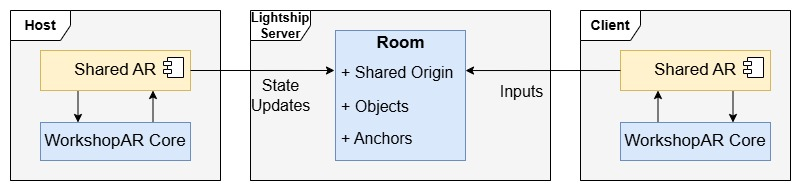
\includegraphics[alt={Figure 4.5},width=0.99\textwidth]{figures/F4-5.jpg}}
    \caption{Integration with Lightship \label{fig:4-5}}
\end{figure}

There is no necessity to go in deep detail about the general architecture of Unity as it is an extensive topic outside the scope of this document that offers little value
to the research. Suffice to say that Unity encourages a modular component approach based around a core engine in charge of the coordination of resources and the
communication with the local device. More information can be found in \textcite{messaoudi_2015}.

As for ARFoundation and Lightship, Figure \ref{fig:4-6} shows a relational model among their most important components, the core development of \emph{WorkshopAR} and the
external elements that interact with the frameworks in the execution of the experience.

\begin{figure}
    \centering{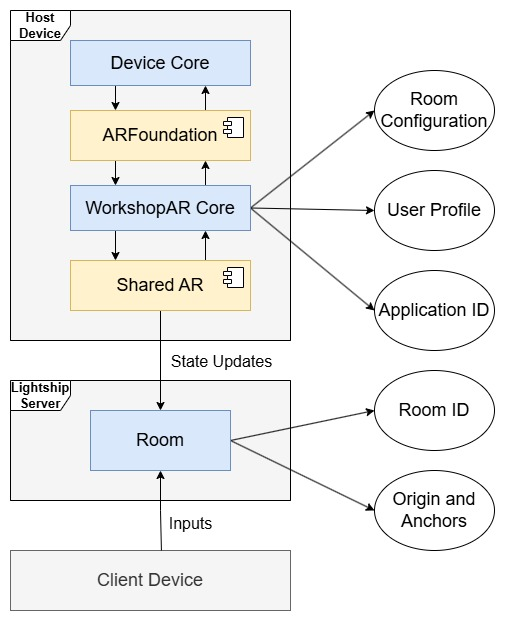
\includegraphics[alt={Figure 4.6},scale=0.75]{figures/F4-6.jpg}}
    \caption{Relational Model with External Frameworks \label{fig:4-6}}
\end{figure}

\subsection{Component Architecture \label{sec:4-3-3}}

\emph{WorkshopAR} uses two major components in its architecture: the \emph{Session Manager}, in charge of the flow of activities in a single session for one participant,
and the \emph{Tracking Manager}, in charge of managing the \ac{AR} interactions. Additional components are added to manage profile data and UI interactions. \emph{WorkshopAR}
relies on the Unity engine framework for deployment in mobile devices, on the ARFoundation package to communicate with the local implementation of \ac{AR} and uses
Lightship in coordination with some proprietary Netcode development to create the shared room and to coordinate interactions.

\emph{WorkshopAR} follows the recommended architecture for general Unity projects, in which the experience follows the execution of one or more scenes which in turn are
composed by a set of game objects. Each object has a specific behaviour determined by its interaction with the engine, other objects and the actions scripted by its
modular components. Following this architecture, \emph{WorkshopAR} creates a \emph{work session} for the users and manages the tracking of all the \ac{AR} elements through
three main objects in a single scene:

\begin{itemize}
    \item The \emph{User Anchor} acts as the visual representation of each participant in the \emph{digital room} and the main control point of each individual action
    through the \emph{Session Manager} component.
    \item The \emph{AR Session} is part of the ARFoundation implementation and provides all the AR functionalities to integrate the scene with the camera image captured in
    the deployment device as well as the detection and management of features in the real space.
    \item The \emph{Network Manager} helps with the implementation of Shared AR and manages all the Netcode used to create the shared experience.
\end{itemize}

Other objects are part to the scene to facilitate the visualisation of UI elements and to manage local data. Figure \ref{fig:4-7} shows a relational model of the
previously described elements in the scene.

\begin{figure}
    \centering{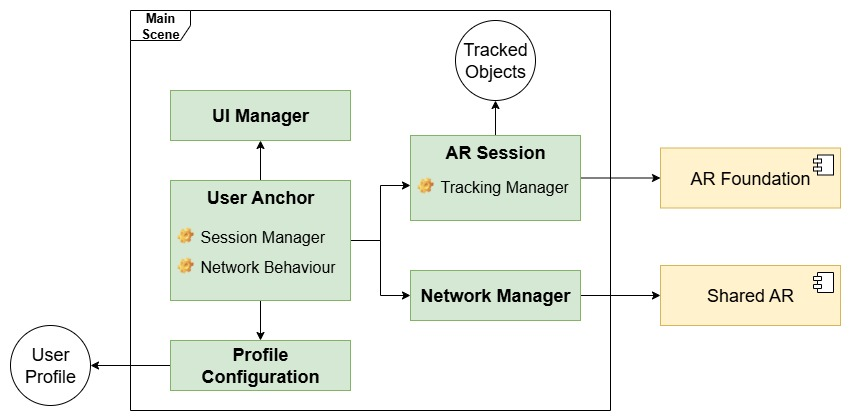
\includegraphics[alt={Figure 4.7},width=0.99\textwidth]{figures/F4-7.jpg}}
    \caption{Unity Scene Relational Model \label{fig:4-7}}
\end{figure}

\subsubsection{Session Manager \label{sec:4-3-3-1}}

The architecture of \emph{WorkshopAR} divides its functionality into two parts: the collaborative session and the \ac{AR} tracking. The \emph{Session Manager} is in charge
of coordinating three elements of the experience: access to the local profile of the user, configuration of the shared room, and coordination of interactions with the room
and with other participants through the network. Other less prominent components are used to provide networking functionalities not managed by Shared AR as well as the
interactions with the UI. The component functionality can be overall described by the following process:

\begin{itemize}
    \item Get the local user profile.
    \item Configure the connection to a room.
    \item Coordinate network behaviours to fulfil the different interactions.
    \item Coordinate interaction calls through the network.
    \item Coordinate local interactions with the necessary data to show in the UI.
\end{itemize}

The \emph{Session Manager} is also associated with the \emph{User Anchor}. The Anchor is the visual and logical representation of the user in the room and provides
different behaviours that show a visual representation  of the user profile (position, name, current task, role) and social cues such as emotes and the user's gaze
direction, all meant to be visual elements for the augmented collaboration design. The \emph{Session Manager} coordinates the creation of \emph{User Anchors} in the
network, bridges local data between users and controls the flow of the session. Figure \ref{fig:4-8} shows a relational model of the most important components involved
with the \emph{Session Manager}.

\begin{figure}
    \centering{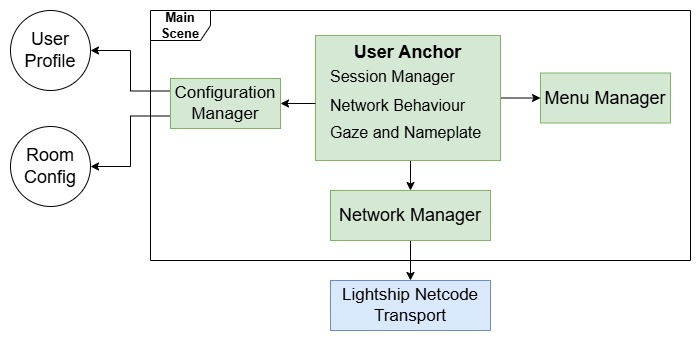
\includegraphics[alt={Figure 4.8},width=0.99\textwidth]{figures/F4-8.jpg}}
    \caption{Session Manager Relational Model \label{fig:4-8}}
\end{figure}

\subsubsection{Tracking Manager \label{sec:4-3-3-2}}

The \emph{Tracking Manager} is part of the \ac{AR} Session game object in charge of controlling the visualisation of digital objects, their behaviour and life cycle. For
purposes of the current prototype of \emph{WorkshopAR}, the available digital objects are play models and annotations. Each object has a unique behaviour that will
interact with the \emph{Session Manager} or the \emph{Tracking Manager} as needed.

The \emph{Tracking Manager} is the bridge between \emph{WorkshopAR} and the ARFoundation framework. It connects all the components needed to create an \ac{AR} scene and
configures the components that provide \ac{AR} functionalities like image composition using the feed of the camera and plane detection in the real space. The manager is
also associated with the XR Origin object, a component needed in the OpenXR framework to abstract the XR device in which the app is going to be deployed. ARFoundation uses
this component to communicate with the functionalities of the mobile device. In summary, the \emph{Tracking Manager} is in charge of:

\begin{itemize}
    \item Initializing the \ac{AR} device.
    \item Managing the behaviour of the main camera.
    \item Managing the digital objects on the scene.
    \item Configuring the \ac{AR} functionalities provided by ARFoundation.
\end{itemize}

The \emph{Tracking Manager} specifically pulls the functionalities related to plane detection and the creation of visual anchors from the ARFoundation framework. The
manager configures these components and keeps track of the game objects used for the visual composition of the scene with the information of the camera. A similar
coordination is done with the \emph{Session Manager}, which keeps track of the life cycle of the objects in the network and the data that needs to be coordinated between
participants. Figure \ref{fig:4-9} shows a relational model of all the components related to the \emph{Tracking Manager}.

\begin{figure}
    \centering{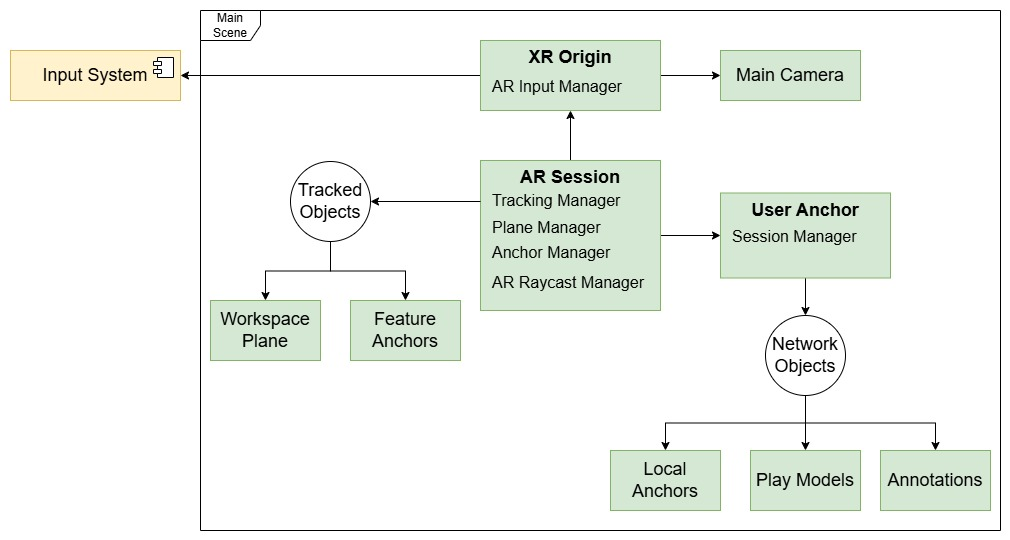
\includegraphics[alt={Figure 4.9},width=0.99\textwidth]{figures/F4-9.jpg}}
    \caption{Tracking Manager Relational Model \label{fig:4-9}}
\end{figure}

\subsubsection{Interaction Pipeline \label{sec:4-3-3-3}}

The connection between the hardware layer of the device and the \emph{digital room} created by \emph{WorkshopAR} follows the architecture proposed by OpenXR. Figure \ref{fig:4-10}
shows the interaction flow between components in case of a local interaction with a digital object, like a play model or an annotation.

\begin{figure}
    \centering{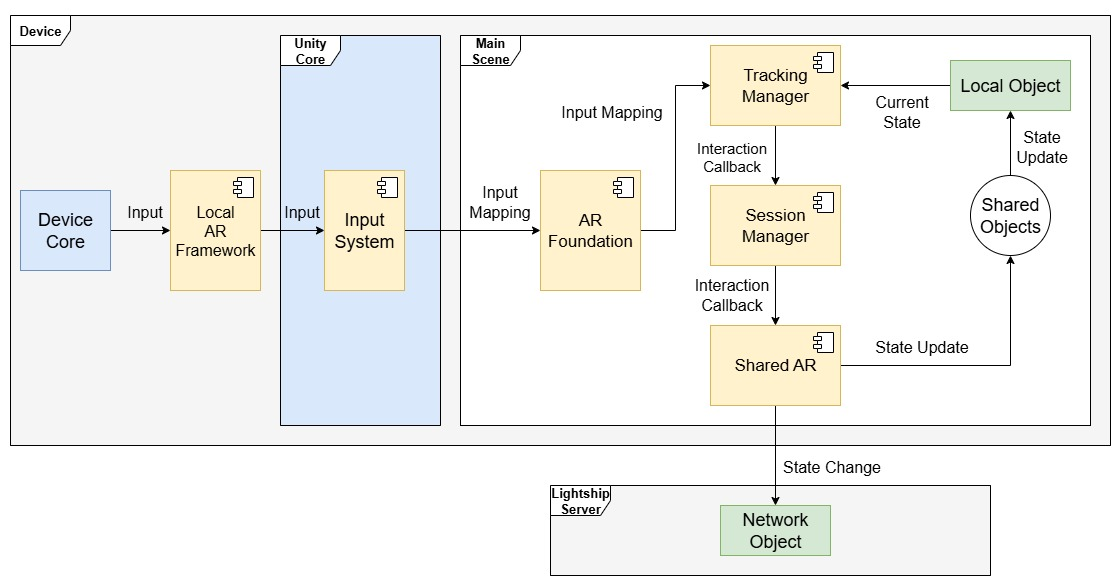
\includegraphics[alt={Figure 4.10},width=0.99\textwidth]{figures/F4-10.jpg}}
    \caption{Device Interaction Flow \label{fig:4-10}}
\end{figure}

The local device is in charge of detecting interactions at a hardware level, most commonly inputs in the touch screen, the relative position of the device (accelerometer,
gyroscope, etc.) and the image feed of the camera. All the input information is then related to the context of the \ac{AR} application thanks to the local framework
present in the device (ARCore or ARkit i.e.) which relays the raw data of the input to the Unity core engine. In here, the ARFoundation framework uses the Input System
provided by Unity to read the raw information of the device and maps it to designated functions implemented by the \emph{Tracking Manager}, which coordinates all the
components, either from ARFoundation or from \emph{WorkshopAR}, needed to respond to the input.

Independent of the components involved in the response, it is first necessary to determine if the interaction changes the state of a shared object. Any change to a shared
object is handled by the \emph{Session Manager}, who coordinates the remote network procedures that propagate the relevant information to all the users, and reacts locally
when a change is received from other user. The \emph{Session Manager} is in charge of updating the state of all the shared objects, while the \emph{Tracking Manager} only
reads the information for visualisation purposes and to manage interactions.

SharedAR supports both server-authoritative and client-authoritative network architectures, as well as the possibility to have dedicated servers or host/client dynamics.
\emph{WorkshopAR} follows a host/client architecture with no dedicated server controlling the experience. The users must decide who is going to act as the host. Then, the
selected user needs to configure the \emph{digital room} and open it, while the other users connect as clients. If the initial host leaves the \emph{digital room}, it is
easy to pass the host authority to any other connected user.

In terms of authority architecture, the host holds server authority for the configuration of the \emph{digital room}, state of the \emph{digital room}, the detected
physical plane used as the shared \emph{workspace}, and the physical features detected as visual anchors. Meanwhile, the \emph{User Anchors}, the play models and the
annotations are client-authoritative, with ownership given to the user that initially spawned the object in the network.

A final consideration is that, despite being designed as a serverless architecture, \emph{WorkshopAR} needs to follow the architecture enforced by SharedAR, which works as
a central server that hosts the shared room and manage the connections of the clients to it. This element is outside the architecture of \emph{WorkshopAR}, and for the end
user, they just need to worry about the connection with the host. Figure \ref{fig:4-11} shows a diagram that represents the main components in the network architecture,
the objects over which each component holds authority and the most important procedures being transmitted over the network.

\begin{figure}
    \centering{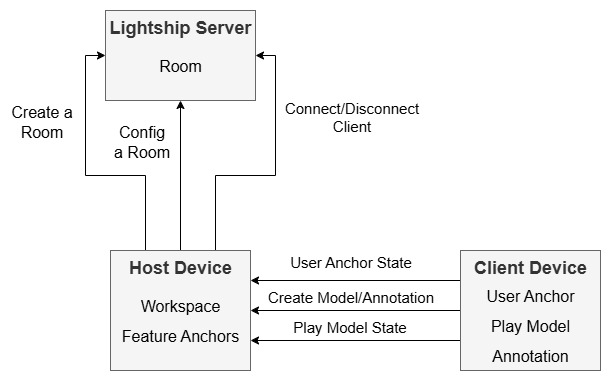
\includegraphics[alt={Figure 4.11},width=0.99\textwidth]{figures/F4-11.jpg}}
    \caption{Network Authority Architecture \label{fig:4-11}}
\end{figure}

In the case that an interaction does not involve digital objects, the pipeline maintains the same architecture. \emph{WorkshopAR} relies on the services provided by
ARFoundation for the detection of features using the camera present in the mobile device, as it is shown in Figure \ref{fig:4-4}. The specific subsystems used by the
prototype are the plane detector, the anchor manager and the \ac{AR} raycast functionalities.

The plane detector is used to identify flat surfaces in the physical space, one of the steps in the configuration of a \emph{digital room}. Similarly, the position of a
digital object can be used to create an anchor in the digital space, which helps improve the quality and stability of the \ac{AR} visualisation. A new anchor is created in
the room every time a new user connects, and these anchors are managed by the host's \emph{Session Manager}. The \ac{AR} raycaster is needed to interact with digital
objects in the \ac{AR} space or with features in the \ac{AR} space created by other subsystems. This is a local operation, so it does not need to be propagated in the
network. Figure \ref{fig:4-12} shows the interactions of the previously described components in the network architecture of \emph{WorkshopAR}.

\begin{figure}
    \centering{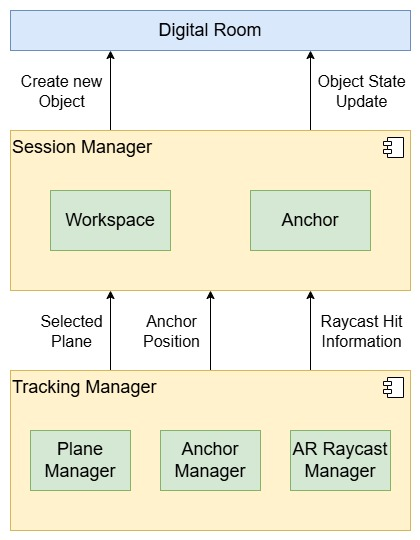
\includegraphics[alt={Figure 4.12},scale=0.75]{figures/F4-12.jpg}}
    \caption{Interaction Pipeline with ARFoundation Subsystems \label{fig:4-12}}
\end{figure}

\subsection{Data Architecture \label{sec:4-3-4}}